\section{Multicapa}
La manera de mejorar nuestros resultados consiste en añadir más capas a nuestra red, las cuales serán capaces de extraer características de las imágenes de entrada. Al añadir nuevas capas, ya no podemos seguir utilizando el algoritmo de aprendizaje del perceptrón. Este algoritmo se basaba en comparar la salida deseada con la obtenida y variar los pesos en consecuencia, cosa que no se puede hacer con el nuevo modelo al no saber cual es la salida que deben tener las neuronas de las capas ocultas. En su lugar, lo que hacemos es establecer una función de coste o pérdida que proporcione un valor del error de la salida final respecto a la deseada y, a continuación, calcular como varía dicho error respecto a cada uno de los pesos de la red. Con ello lo que buscamos es descender por el gradiente de este error hacia los valores de los pesos que lo minimizan.

\begin{equation}
    E = \frac{1}{2} \sum_{n} (t^n-y^n)^2
\end{equation}

\begin{equation}
    \Delta w_{ij} = - \eta \frac{\delta E}{\delta w_{ij}}
\end{equation}

En este primer modelo multicapa, mido esta pérdida usando la función del error cuadrático medio para un conjunto de $n$ ejemplos de entrada, tal y como se puede ver en la ecuación 3. En mi caso, al realizar entrenamiento \textit{online}, esta $n$ es 1. La ecuación 4 muestra la manera de calcular el incremento que se debe aplicar a cada peso para disminuir el error obtenido.

Como podemos apreciar, se aplica una constante $\eta$ conocida como la tasa de aprendizaje. Esta constante se encarga de controlar los "saltos" que da nuestro modelo por el gradiente del error. Conforme entreno el modelo, reduzco esta tasa para evitar que las actualizaciones de los pesos sean demasiado grandes y nos pasemos del mínimo objetivo. La ecuación 5 es la que utilizo para calcular la tasa de aprendizaje para una época $t$ en función de la tasa inicial $\eta_0$.

\begin{equation}
    \eta_t = \frac{\eta_0}{1 + \frac{t}{2}}
\end{equation}

Si las neuronas de estas nuevas capas ocultas usan también una función de activación lineal como la de la ecuación 2, seguiríamos teniendo un clasificador lineal como ocurría con el perceptrón. Es por ello que debemos introducir una función de activación no lineal, que en mi caso será la función logística (ecuación 6).

\begin{equation}
    y_i = \frac{1}{1 + e^{-z_i}}
\end{equation}

Construyo entonces una red con una capa oculta de 256 neuronas y una capa de salida de 10 neuronas, todas ellas usando la función logística como función de activación. Cambian las salidas, que ya no van a ser 0 o 1, si no que son valores entre 0 y 1, por lo que interpretamos que la clase predicha por el modelo es la salida más alta. Obtengo los siguientes resultados:

\begin{center}
    \begin{tabular}{ |c|c|c|c| } 
        \hline
        $\acute Epocas$ & $Tiempo$ & $Error_{train}$ & $Error_{test}$ \\
        \hline
        10       & 1631,12s &  1,57\%         & 2,89\%         \\
        \hline
    \end{tabular}
\end{center}

Para intentar mejorar estos resultados, cambio la capa de salida por una capa \textit{softmax}, que es más apropiada para los problemas de clasificación en los que hay más de dos clases. Las neuronas de la capa de salida van a utilizar entonces la función de activación \textit{softmax} (ecuación 7), la cual hace que la suma de todas las salidas sea igual a 1. La salida de cada neurona va a ser entonces una probabilidad de que la entrada pertenezca a la clase que representa la neurona.

\begin{equation}
    y_i = \frac{e^{z_i - c}}{\sum_{j=1}^n e^{z_j - c}}
\end{equation}

Al usar exponenciales, los valores pueden dispararse y he llegado a experimentar problemas de \textit{overflow}. Es por ello que uso la mayor de las entradas netas de la capa de salida como constante $c$ para controlar el tamaño de estas exponenciales.

Como uso esta nueva función, debo cambiar también la función de coste del modelo por la de la entropía cruzada (ecuación 8).

\begin{equation}
    C = - \sum_j t_j \log y_j
\end{equation}

Usando una capa oculta de 256 unidades logísticas y una capa de salida \textit{softmax} de 10 clases, obtengo los siguientes resultados:

\begin{center}
    \begin{tabular}{ |c|c|c|c|c| } 
        \hline
        $\eta_0$ & $\acute Epocas$ & $Tiempo$ & $Error_{train}$ & $Error_{test}$ \\
        \hline
        0,5      & 10       & 1666,71s &  7,94\%         & 8,92\%         \\
        \hline
        0,1      & 10       & 1647,90s &  0,11\%         & 2,51\%         \\
        \hline
        0,1      & 30       & 4966,82s &  0,0083\%       & 2,48\%         \\
        \hline
    \end{tabular}
\end{center}

En el primer experimento obtuve resultados peores que los obtenidos con el modelo anterior. Esto se debía a que estaba usando una tasa de aprendizaje inicial demasiado elevada. Al reducirla, alcancé en el mismo número de épocas el 2,51\% de error sobre el conjunto de prueba. En la siguiente gráfica se puede apreciar cómo va descendiendo la tasa de error sobre el conjunto de entrenamiento al avanzar las épocas para estas dos tasas de aprendizaje iniciales. 

\begin{center}
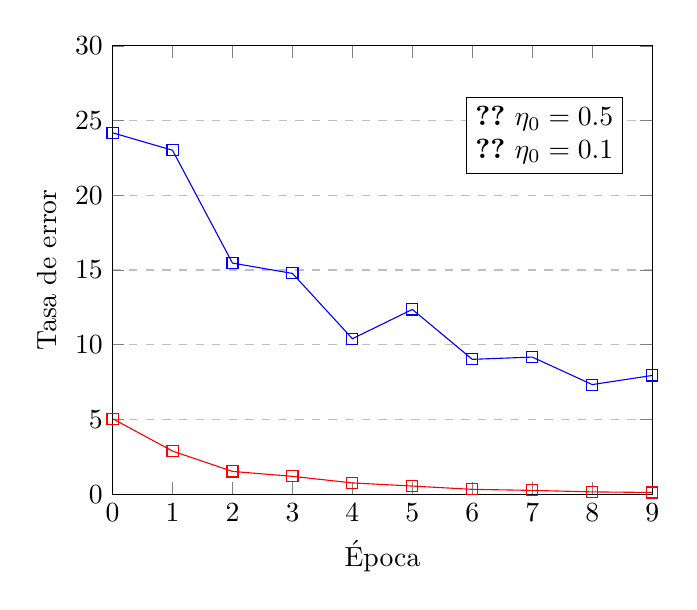
\begin{tikzpicture}
\begin{axis}[
    xlabel={Época},
    ylabel={Tasa de error},
    xmin=0, xmax=9,
    ymin=0, ymax=30,
    xtick={0,1,2,3,4,5,6,7,8,9},
    ytick={0,5,10,15,20,25,30},
    ymajorgrids=true,
    grid style=dashed,
]
 
\addplot[
    color=blue,
    mark=square,
    ]
    coordinates {
    (0,24.18)(1,23.01)(2,15.46)(3,14.77)(4,10.40)(5,12.36)(6,9.02)(7,9.17)(8,7.33)(9,7.94)
    };
\label{p1}
    
\addplot[
    color=red,
    mark=square,
    ]
    coordinates {
    (0,5.05)(1,2.88)(2,1.52)(3,1.19)(4,0.75)(5,0.54)(6,0.32)(7,0.25)(8,0.15)(9,0.11)
    };
\label{p2}
    
\node [draw,fill=white] at (rel axis cs: 0.8,0.8) {\shortstack[l]{
\ref{p1} $\eta_0 = 0.5$ \\
\ref{p2} $\eta_0 = 0.1$}};
 
\end{axis}
\end{tikzpicture}
\end{center}

Aumentando el número de épocas, conseguimos disminuir el error sobre el conjunto de entrenamiento casi al 0\%, pero el error sobre el conjunto de prueba apenas se ve afectado.